\section{Auswertung}
\label{sec:Auswertung}
Eine Leermessung ist in Abbildung \ref{fig:Leer} zu sehen. Die Comptonkante und der Photopeak liegen bei $C\approx \SI{478}{\kilo\eV}$ und 
$P\approx\SI{662}{\kilo\eV}$ \cite{Lit_Wert_Comp}.
\begin{figure}
    \centering
    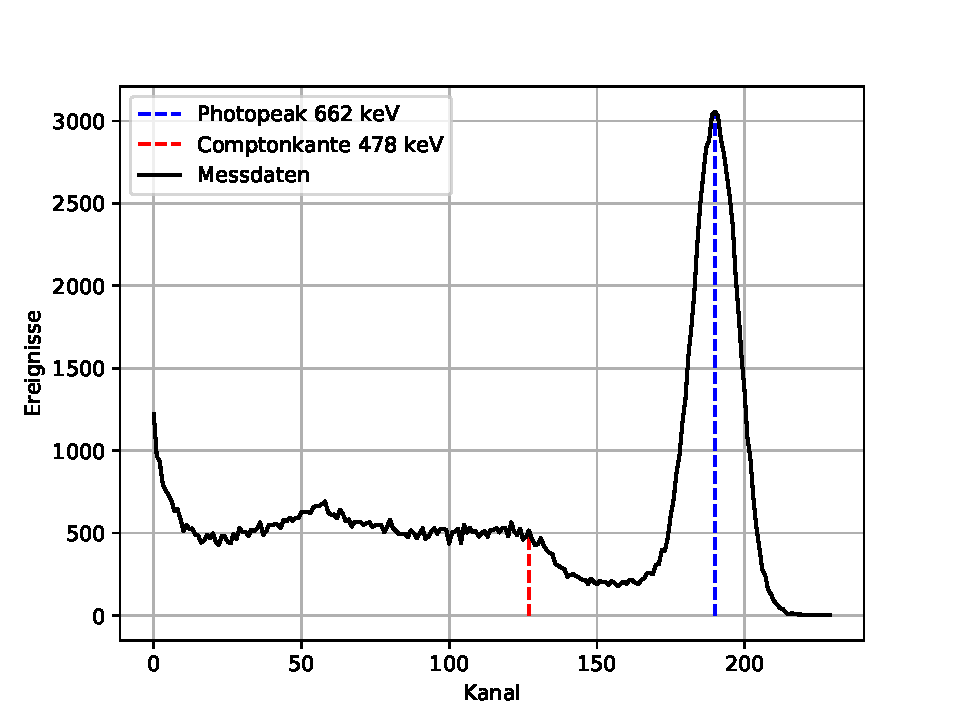
\includegraphics[]{figure/Leer.pdf}
    \caption{Spektrum des $\ce{^137Cs}$-Strahler ohne Würfel.}
    \label{fig:Leer}
\end{figure}
\subsection{Bestimmung der Absorptionskoeffizienten}
Um die Absorptionskoeffizienten zu bestimmen müssen zunächst die $I_0$-Werte bestimmt werden. 
Hierfür wird der Würfel 1 genommen, der nur aus der Aluminiumhülle besteht. Es werden drei 
verschiedene $I_0$-Werte gemessen, für die Diagonale $D$, Nebendiagonale $ND$ und für die seitenparallele Grade $SG$.
Die $I_0$-Werte sind in Tabelle \ref{tab:I_0} aufgelistet.
\FloatBarrier
\begin{table}
    \centering
    \caption{Messdaten für die Bestimmung der $I_0$-Werte und die dazugehörigen $I_0$-Werte.}
    \label{tab:I_0}
    \begin{tabular}{c c c c}
        \toprule
        Ausrichtung&Peakinhalt $C$&Zeit $\Delta t \,/\,\SI{}{\second}$&Zählrate $I_0 \,/\,\SI{}{1\per\second}$\\
        \midrule
        $D$ &$\num{10396(300)}$&$\num{126.44}$&$\num{82.2(24)}$\\
        $ND$&$\num{14398(247)}$&$\num{117.90}$&$\num{122.1(21)}$\\
        $SG$&$\num{12927(271)}$&$\num{119.60}$&$\num{108.1(23)}$\\
        \bottomrule
    \end{tabular}
\end{table}
\FloatBarrier
\subsection{Würfel 1 und 2}
Die beiden Würfel 1 und 2 bestehen aus je einem Material, daher werden nur drei Werte gemessen.
Die Messdaten sind in Tabelle \ref{tab:Würfel_1_2} aufgelistet.
\FloatBarrier
\begin{table}
    \centering
    \caption{Messdaten für die Bestimmung der Absorptionskoeffizienten der Würfel 1 und 2.}
    \label{tab:Würfel_1_2}
    \begin{tabular}{c c c c c c c}
        \toprule
        &\multicolumn{3}{c}{Würfel 1}&\multicolumn{3}{c}{Würfel 2}\\
        \cmidrule(lr){2-4}\cmidrule(lr){5-7}
        Ausrichtung&$C$&$\Delta t \,/\,\SI{}{\second}$&$I \,/\,\SI{}{1\per\second}$&$C$&$\Delta t \,/\,\SI{}{\second}$&$I \,/\,\SI{}{1\per\second}$\\
        \midrule
        $D$ &$\num{5096(109)}$&$\num{300}$&$\num{16.6(5)}$&$\num{19747(237)}$&$\num{210.88}$&$\num{93.6(11)}$\\
        $ND$&$\num{4984(157)}$&$\num{300}$&$\num{16.9(4)}$&$\num{22765(246)}$&$\num{208.98}$&$\num{108.9(12)}$\\
        $SG$&$\num{7662(142)}$&$\num{300}$&$\num{25.5(5)}$&$\num{19147(225)}$&$\num{178.60}$&$\num{107.2(13)}$\\
        \bottomrule
    \end{tabular}
\end{table}
\FloatBarrier
Mit den Gleichungen
\begin{equation*}
    \mu_{\text{j}}= \frac{\log{\left(\frac{I_0}{I_\text{j}}\right)}}{d_{\text{j}}}
\end{equation*} 
und den Messdaten aus Tabelle \ref{tab:Würfel_1_2} und \ref{tab:I_0} können die Absorptionskoeffizienten bestimmt werden. 
Die Weglängen $d_{\text{j}}$ betragen
\begin{gather*}
    d_{D} =\frac{3}{\sqrt{2}}\SI{}{\centi\meter}\\
    d_{ND}=\frac{2}{\sqrt{2}}\SI{}{\centi\meter}\\
    d_{SG}=\SI{3}{\centi\meter}.
\end{gather*}
Die berechneten Absorptionskoeffizienten der beiden Würfel sind in Tabelle \ref{tab:Absorptionskoeffizienten_1_2} aufgelistet.
\FloatBarrier
\begin{table}
    \centering
    \caption{Absorptionskoeffizienten der Würfel 1 und 2, gemittelt und für jede einzelne Ausrichtung.}
    \label{tab:Absorptionskoeffizienten_1_2}
    \begin{tabular}{c c c}
        \toprule
        &Würfel 1&Würfel 2\\
        \cmidrule(lr){2-2}\cmidrule(lr){3-3}
        Ausrichtung&$\mu \,/\,\SI{}{1\per\centi\meter}$&$\mu \,/\,\SI{}{1\per\centi\meter}$\\
        \midrule
        D &$\num{0.466(6)}$&$\num{-0.099(11)}$\\
        ND&$\num{0.565(15)}$&$\num{0.063(5)}$\\
        SG&$\num{0.481(9)}$&$\num{0.003(8)}$\\
        \midrule
        gemittelt&$\num{0.504(6)}$&$\num{0.033(5)}$\\
        \bottomrule
    \end{tabular}
\end{table}
\FloatBarrier
Für den Mittelwert aus Tabelle \ref{tab:Absorptionskoeffizienten_1_2} wird der negative Wert nicht beachtet da dieser unphysikalisch ist,
darauf wird in der Diskussion eingegangen.
\subsection{Würfel 4}
Die Absorptionskoeffizienten $\mu_{\text{j}}$ werden für Würfel 4 mit der Gleichung \eqref{??}[Gleichung für $\mu$] bestimmt.
Die Elemente der diagonalen Gewichtsmatrix $W$ werden mithilfe der gaußschen Fehlerfortpflanzung bestimmt.
\begin{equation*}
    W_{\text{jj}}= \left(\sqrt{\left(\frac{\sigma_{I_0}}{I_0}\right)^2+ \left(\frac{\sigma_{I_j}}{I_j}\right)^2}\right)^{-1}
\end{equation*}
Die Messdaten für die Bestimmung der Absorptionskoeffizienten sind in Tabelle \ref{tab:Messdaten_Würfel4} aufgelistet.
\FloatBarrier
\begin{table}
    \centering
    \caption{Messdaten und die damit bestimmten Elemente der Gewichtsmatrix für die Bestimmung der Absorptionskoeffizienten des Würfels 4, jede Ausrichtung wurde $\SI{300}{\second}$ lang gemessen. Die Ausrichtungen sind wie in Abbildung \ref{fig:??}[Schematische abbidlung der Ausrichtung]}
    \label{tab:Messdaten_Würfel4}
    \begin{tabular}{c c c c}
        \toprule
        Ausrichtung $j$&$C$&$I\,/\,\SI{}{1\per\second}$&$W_{\text{jj}}$\\
        \midrule
        $\num{1}$&$\num{24609}$&$\num{82.0}$ &$\num{32.2}$\\
        $\num{2}$&$\num{16380}$&$\num{54.6}$ &$\num{44.6}$\\
        $\num{3}$&$\num{25913}$&$\num{86.4}$ &$\num{32.5}$\\
        $\num{4}$&$\num{16964}$&$\num{56.5}$ &$\num{38.6}$\\
        $\num{5}$&$\num{17465}$&$\num{58.2}$ &$\num{39.1}$\\
        $\num{6}$&$\num{14876}$&$\num{49.6}$ &$\num{35.7}$\\
        $\num{7}$&$\num{21195}$&$\num{70.6}$ &$\num{31.2}$\\
        $\num{8}$&$\num{16389}$&$\num{54.6}$ &$\num{43.6}$\\
        $\num{9}$&$\num{23458}$&$\num{78.2}$ &$\num{31.7}$\\
        $\num{10}$&$\num{12895}$&$\num{43.0}$&$\num{32.4}$\\
        $\num{11}$&$\num{15569}$&$\num{51.9}$&$\num{36.9}$\\
        $\num{12}$&$\num{17778}$&$\num{59.3}$&$\num{39.4}$\\
        \bottomrule
    \end{tabular}
\end{table}
\FloatBarrier